\section{Zielsetzung}
Bei dem Versuch sollen die Leerlaufspannung und der Innenwiderstand einer Monozelle
auf verschiedene Weisen bestimmt werden. Zudem soll auch ein Sinus- und Rechteck-
Spannungsgenerator zur Bestimmung dieser Größen verwendet werden.

\section{Theorie}
Jede Spannungsquelle, unter welcher man ein Gerät versteht was eine zeitlich konstante
elektrische Leistung iefert, besitzt eine feste Leerlaufspannung $\text{U}_0$, welche
anliegt wenn kein Strom fließt. Sobald die Spannungsquelle in einen geschlossenen
Stromkreis eingebaut wird und somit ein Strom fließt,
liefert diese nur noch die Klemmspannung $\text{U}_k$, welche stets kleiner als
die Leerlaufspannung ist, was sich über das zweite Kirchhoffsche Regel
\begin{equation}
  \sum_i U_i = 0
\end{equation}
beweisen lässt. Dies liegt daran, dass jede Spannungsquelle einen Innenwiderstand
$\text{R}_i$ besitzt, sodass bei einem zusätzlich in Reihe geschalteten Widerstand
$\text{R}_a$ gilt:
\begin{equation}
  U_0 = I\cdot R_a + I\cdot R_I \iff I\cdot R_a = U_k = U_0 - I\cdot R_I
\end{equation}
Dies lässt sich auch an einem Ersatzschaltbild darstellen, wobei die reale
Spannungsquelle in eine ideale Spannungsquelle (ohne Innenwiderstand) und einen
in Reihe geschalteten externen Widerstand aufgeteilt ist, wie in Abbildung
\ref{fig:schalt1} zu sehen ist.
\begin{figure}[H]
  \centering
  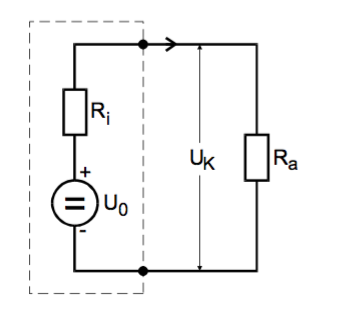
\includegraphics[height=6cm]{schalt1.png}
  \caption{Ersatztschalbild einer Spannungsquelle mit Widerstand \cite{skript}}
  \label{fig:schalt1}
\end{figure}
\noindent Um die Leerlaufspannung zu messen, sollte also ein möglichst hochohmiges Voltmeter
verwendet werden, da somit der Strom I sehr klein wird und der Term
$ \text{I}\cdot \text{R}_I \to 0 $ läuft, sodass dieser vernachlässigbar ist und
$ \text{U}_k \approx \text{U}_0 $ gilt. \\
\noindent Eine weitere Folge ist, dass die entnommene elektrische Leistung nicht
beliebig hoch werden kann sondern begrenzt ist, da diese durch die Formel
\begin{equation}
  N(R_a) = I^2 \cdot R_a
\end{equation}
gegeben ist und bei $\text{R}_I = \text{R}_a$ ein Maximum durchläuft. \\
\noindent Falls $\text{R}_a$ entsprechend gewählt wird, wird dies auch
Leistungsanpanssung genannt, was vor allem in der Nachrichten- und Mess-
Technik Anwendung findet.
